\documentclass{article}
\usepackage[utf8]{inputenc}
\usepackage{amsmath}
\usepackage{graphicx}
\graphicspath{ {./Grafics/}}

\title { Teoria Geoc: Basic Tools}
\date { Quadrimestre Tardor 2019-2020}
\author {Pol Renau Larrod\'e}

\begin{document}
  \maketitle
  \newpage

  \section {DESCRIBING AND IMPLEMENTING BASIC GEOMETRIC OBJECTS}

    Homogeneous cordinates are very usefull in practice, allows us to calculate a lot of things.

    {\it Point:}
    \[ (x,y) \Leftrightarrow (x:y:1) \]

    {\it Line:}
    \[ ax + bx +c =0 \Leftrightarrow (a:b:c) \]


    Incidence pont-line:
      \begin{center} p = (x:y:1) lies in l = (a:b:c) \Leftrightarrow (a,b,c)  (x,y,1) = 0 \end{center}

    Line through two points:
      \begin{center}p and q lies in l \Rightarrow l = p x q \end{center}

    Intersecting two lines:
      \begin{center} p lies in l1 and l2 \Rightarrow p = l1 x l2 \end{center}

    Parallel lines:
      \begin{center} l1 \parallel l2 \Leftrightarrow l1 x l2  = (x,y,0) \end{center}

    Identical lines or points:
    \begin{center}  Make cross product between them is 0: l1 x l2 = (0,0,0) \end{center}

    \section {Orientation tests}

        Given 3 points in the plane p,q,r a robously decide whether r lies to the  left, right or oriented to pq line.
        \\


        \begin{vmatrix}
          q_x - p_x & r_x -p_x \\
          q_y -p_y & r_y - p_y
        \end{vmatrix}
        \\
        The result of this determinant, determine, if lies to left, right or oriented to line.
        \\

        If determinant menor 0 lies to left
        \\

        If determinant major 0 lies to right
        \\

        If determinant = 0 lies oriented to pq.

        \\

        The same operation can be do it for calculate relative position of point-plane:

        \begin{center}
        det(x,a,b,c), where a,b,c are points of plane $\pi$
        \end{center}

      \newpage
      This can be aplicated to know if a point lies in to circle or not. Cause is known that a circle is a paraboloid intersect by a determinate plane.

      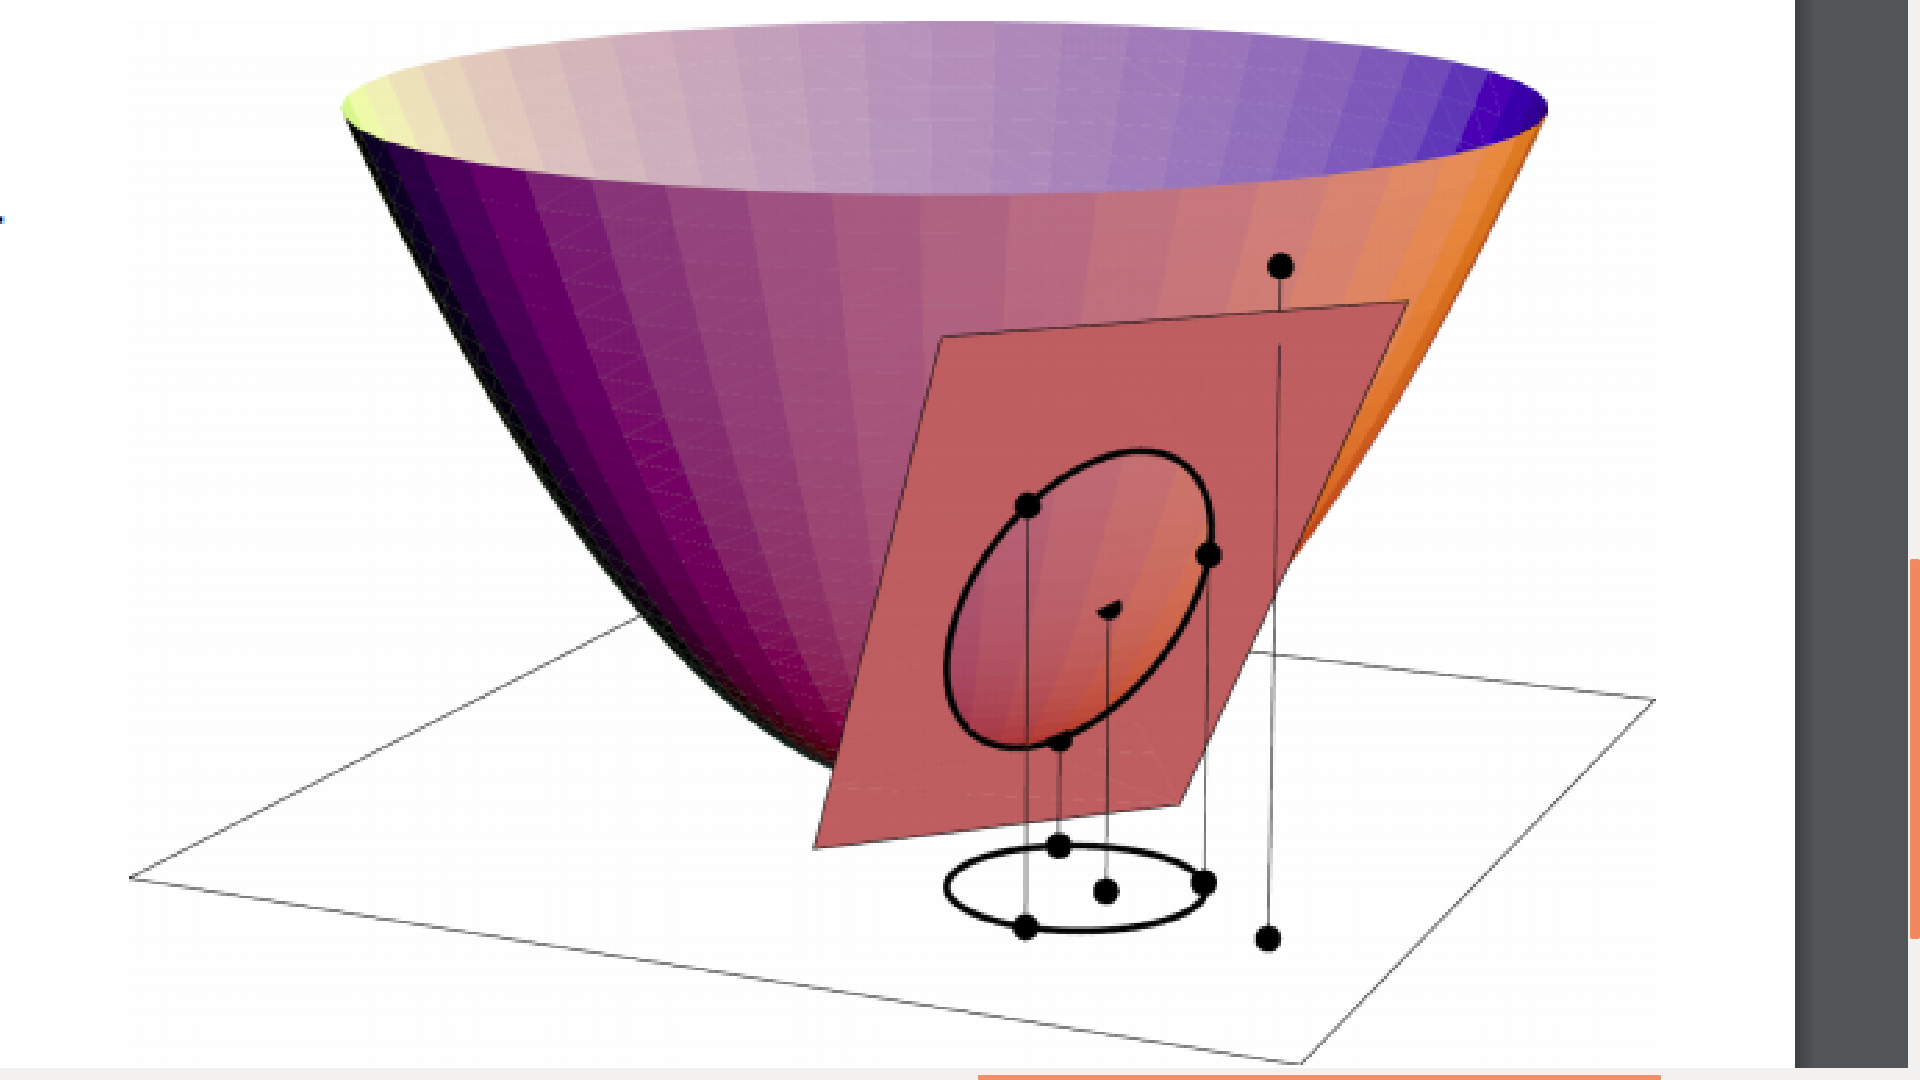
\includegraphics[width=\textwidth]{Paraboloid}



      Orientation test can be aplicated in test polygons. For know if line intersect whith polygon, if point lies into polygon, or to calculate suporting lines( given a point we draw 2 lines that all points lies to the left, and other that all point lies to the right)
      \\ This test have a O(n) cost, but if the polygon is convex the cost is reduced to O(log(n))




\end{document}
